\documentclass[hess, manuscript]{copernicus}

\usepackage{makecell} \usepackage{multirow} %AM for tables
\usepackage{hyperref}
\usepackage[title]{appendix}
\usepackage{booktabs}
\usepackage{longtable}

\newcommand{\appropto}{\mathrel{\vcenter{
      \offinterlineskip\halign{\hfil$##$\cr
        \propto\cr\noalign{\kern2pt}\sim\cr\noalign{\kern-2pt}}}}}

\begin{document}

\title{When does vapor pressure deficit drive or reduce
  evapotranspiration?}
\Author[1]{Adam}{Massmann}
\Author[1]{Pierre}{Gentine}
\Author[1,2]{Changjie}{Lin}


\affil[1]{Department of Earth and Environmental Engineering,
  Columbia University, New York, NY 10027}
\affil[2]{State Key Laboratory of Hydroscience and Engineering, Department of Hydraulic
  Engineering, Tsinghua University, Beijing, CN 100084}

\runningtitle{When does VPD drive or reduce ET?}

\runningauthor{A. Massmann}

\correspondence{Adam Massmann (akm2203@columbia.edu)}


\firstpage{1}

\maketitle

\begin{abstract}
Increasing vapor pressure deficit (VPD) increases atmospheric demand
for water, and vapor pressure deficit is expected to rise with
increasing greenhouse gases. While increased evapotranspiration (ET)
in response to increased atmospheric demand seems intuitive, plants
are capable of reducing ET in response to increased VPD by closing
their stomata, in an effort to conserve water. Here we examine which
effect dominates response to increasing VPD: atmospheric demand and
increases in ET, or plant physiological response (stomata closure) and
decreases in ET. We use Penman-Monteith, combined with semi-empirical
optimal stomatal regulation theory and underlying water use
efficiency, to develop a theoretical framework for understanding how
ET responds to increases in VPD. The theoretical ET response to VPD
over a range of reasonable environmental conditions and plant
characteristics varies from a strong decrease in ET in response to
increasing VPD (water conservative) to a strong increase in ET in
response to VPD (water intensive), highlighting the diversity of plant
water regulation strategies.

The ET response varies due to: 1) climate, with tropical and temperate
climates more likely to exhibit a positive ET response to increasing
VPD than boreal and arctic climates; 2) photosynthesis strategy, with
C3 plants more likely to exhibit a positive ET response than C4
plants; and 3) due to plant type, with crops more likely to exhibit a
positive ET response, and shrubs and gymniosperm trees more likely to
exhibit a negative ET response. These results, derived from previous
literature connecting plant parameters to plant and climate
characteristics, highlight the utility of our simplified framework for
understanding complex land atmosphere systems in terms of idealized
scenarios. In this example we consider a scenario in which
evapotranspiration responds to VPD only, which is otherwise
challenging to assess in an environment where everything co-evolves.

\end{abstract}

\introduction
Vapor pressure deficit (VPD) is expected to rise over continents in
the future due to the combination of increased temperature and,
depending on region, decreased relative humidity
\citep{Byrne_2013}. Increases in VPD increase the atmospheric demand
for evapotranspirated water \citep{Penman_1948, Monteith_1965}, but
also stress plant stomata \citep{Leuning_1990, MEDLYN_2011}.

The opposing effects of increased atmospheric demand and higher
stomatal stress lead to two possible perspectives for how
evapotranspiration (ET) responds to shifts in VPD. The first, a
hydrometeorological perspective, is that higher VPD increases
atmospheric demand for water from the land surface, and this drives an
increase in evapotranspiration (ET). This perspective is particularly
relevant because potential evapotranspiration (PET), which is used in
many drought indices and hydrometeorological studies
\citep[e.g.,][]{Heim_2002, Scheff_2015}, typically only quantifies
changes in atmospheric demand and fails to account for ecosystem
response \citep{Swann_2016}. In reality, plants' stomata have evolved
to optimally regulate the exchange of water and carbon, and tend to
partially close in response to increased atmospheric dryness
\citep{Farquhar_1978, Ball_1987, Leuning_1990, MEDLYN_2011}. This
leads to a plant physiology perspective, in which an increase in VPD,
particularly in well-watered soil conditions, may actually correspond
to a decrease in ET because of stomatal closure
\citep[e.g.][]{Rigden_2017}.  In other words, the question ``When does
VPD drive or reduce ET?'' can be related to whether plant regulation
or atmospheric demand dominates ET response.

The ET response to changes in VPD alters water partitioning between
the soil and atmosphere. If ecosystem plant response reduces ET with
atmospheric drying then soil moisture will be better conserved. This
represents a sensible evolutionary strategy to cope with aridity: save
water for periods when atmospheric demand for water is relatively low,
and atmospheric carbon can be accessed with a relatively smaller cost
in water loss. If instead stomata were fully passive \citep [similar
to soil pores, e.g. ][]{Or_2013}, increased atmospheric aridity would
strongly reduce soil moisture \citep{Berg_2017}. This could further
increase aridity as low soil moisture levels increases the Bowen
ratio, leading to increased temperature and atmospheric drying
\citep[][]{Bouchet_1963, Morton_1965, Brutsaert_1999, Ozdogan_2006,
  Salvucci_2013, Gentine_2016, Berg_2016}. Therefore, passive
regulation and a lack of soil moisture conservation does not seem to
be a sensible strategy for plants from an evolutionary standpoint.

As a counterpoint, one may argue that increases in ET with increasing
VPD could increase the likelihood of precipitation
\citep[e.g.,][]{Findell_2011}. However, increases in ET do not always
guarantee an increased likelihood of precipitation, which depending on
environmental conditions could cause a decrease in the likelihood of
precipitation \citep[][]{Gentine_2013}. Furthermore, any increases in
precipitation are likely to be non-local, such that plants giving up
water to the atmosphere are not guaranteed to reap the benefits of
water returned from the atmosphere to the soil. Using this subjective
logic, from an ecosystem evolutionary perspective, water stored in
soil seems to be worth much more than the chance of water returned as
precipitation.

We can use intuition about plant water conservation strategy to
hypothesize about ET response to changes in VPD. Plants and ecosystems
that evolved to conserve water, such as arid shrubs or savannah,
should be more likely to reduce ET with increasing VPD, and plants
that have evolved or have been engineered to care little about water,
such as crops, will be more likely to increase ET with increasing
VPD. Atmospheric conditions must matter as well. At the ecosystem
scale, there are limits to plant water conservation strategies. As
atmospheric demand for water (VPD) increases, ecosystems should begin
to reach their water conservation limits and might not be able to
entirely limit ET flux to the atmosphere. At this stage any further
increase in VPD will most likely drive a (limited) increase in ET,
because the increase in atmospheric demand for water overwhelms the
limited plant response to conserve water.

The objective of the present manuscript is to use reasonable
approximations established in prior research as a tool to develop a
framework for understanding plant response to atmospheric drying and
evaluating the VPD dependence of ET. This framework will aid
interpretation of observations, full complexity models, and facilitate
the disentanglement of complex land-atmosphere feedbacks. In the past,
similar approaches were used to understand interactions between
stomatal conductance, evapotranspiration and the environment
\citep[e.g.,][]{Jarvis_1986, Mcnaughton_1991}. However, at the time
researchers' understanding of the form of VPD's effect on plant
physiology was limited, so they could not explore the sensitivity of
ET to VPD, including VPD's effect on stomatal conductance and plant
function.

Recent results have drastically improved our understanding of VPD's
impact on physiology, especially at the leaf
level. \citet{MEDLYN_2011} developed a model for leaf-scale stomatal
conductance ($g_s$), including VPD response, by combining an optimal
photosynthesis theory \citep{Cowan_1977} with an empirical approach,
and extended use of this model to the ecosystem scale in
\citet{Medlyn_2017}. Additionally, \citet{Zhou_2014} demonstrated that
a quantity underlying water use efficiency $\left(uWUE = \frac{GPP\;
\sqrt{VPD}}{ET}\right)$ properly captures a constant relationship
between GPP, ET, and VPD over a diurnal cycle at the ecosystem
scale. uWUE is also relatively well conserved in the growing season
across space and time, within a PFT \citep{Zhou_2015}. While stomatal
conductance parameterizations and uWUE greatly simplify complex plant
physiological processes, they still capture ecosystem behavior for
vegetated surfaces \citep{Medlyn_2017, Zhou_2014}, and are novel tools
to transparently develop intuition for the behavior of complex,
multiscale ecohydrologic systems.

In this manuscript, we leverage uWUE and recent developments in
stomatal conductance parameterizations \citep{MEDLYN_2011} to derive
the theoretical one-way response of ET to VPD with other environmental
variables properly controlled for, i.e. we develop a framework for
evaluating the partial derivative of ET with respect to VPD. For the
first time, we explicitly include VPD's full effect on stomatal
conductance, including its impact on photosynthesis. We explore the
range of possible ET responses to VPD, given parameters previously
established in peer reviewed literature. Additionally, we show the
sensitivity of the ET-VPD relationship to model and framework choice,
highlighting the importance of: 1) future research on stomatal
conductance and ecosystem scaling, and 2) thoughtful selection of
photosynthesis and stomatal conductance model in more sophisticated
land surface and earth system models.


\section{Introduction}

Vapor pressure deficit (VPD) is expected to rise over continents in
the future due to the combination of increased temperature and,
depending on region, decreased relative humidity
\citep{Byrne_2013}. Increases in VPD increase the atmospheric demand
for evapotranspirated water \citep{Penman_1948, Monteith_1965}, but
also stress plant stomata \citep{Leuning_1990, MEDLYN_2011}.

The opposing effects of increased atmospheric demand and higher
stomatal stress lead to two possible perspectives for how
evapotranspiration (ET) responds to shifts in VPD. The first, a
hydrometeorological perspective, is that higher VPD increases
atmospheric demand for water from the land surface, and this drives an
increase in evapotranspiration (ET). This perspective is particularly
relevant because potential evapotranspiration (PET), which is used in
many drought indices and hydrometeorological studies
\citep[e.g.,][]{Heim_2002, Scheff_2015}, typically only quantifies
changes in atmospheric demand and fails to account for ecosystem
response \citep{Swann_2016}. In reality, plants' stomata have evolved
to optimally regulate the exchange of water and carbon, and tend to
partially close in response to increased atmospheric dryness
\citep{Farquhar_1978, Ball_1987, Leuning_1990, MEDLYN_2011}. This
leads to a plant physiology perspective, in which an increase in VPD,
particularly in well-watered soil conditions, may actually correspond
to a decrease in ET because of stomatal closure
\citep[e.g.][]{Rigden_2017}.  In other words, the question ``When does
VPD drive or reduce ET?'' can be related to whether plant regulation
or atmospheric demand dominates ET response.

The ET response to changes in VPD alters water partitioning between
the soil and atmosphere. If ecosystem plant response reduces ET with
atmospheric drying then soil moisture will be better conserved. This
would seem a sensible evolutionary strategy to cope with aridity. If
stomata were fully passive \citep [similar to soil pores,
e.g. ][]{Or_2013}, increased atmospheric aridity would strongly reduce
soil moisture \citep{Berg_2017}. In turn, this would further increase
aridity as low soil moisture levels increase the Bowen ratio, and
cause increased temperature and atmospheric drying
\citep[][]{Bouchet_1963, Morton_1965, Brutsaert_1999, Ozdogan_2006,
  Salvucci_2013, Gentine_2016, Berg_2016}. This however would not seem
to be a sensible strategy for plants from an evolutionary
standpoint. As a counterpoint, one may argue that increases in ET with
increasing VPD could increase the likelihood of precipitation
\citep[e.g.,][]{Findell_2011}. However, increases in ET do not always
guarantee an increased likelihood of precipitation, which depending on
environmental conditions could cause a decrease in the likelihood of
precipitation \citep[][]{Gentine_2013}. Furthermore, any increases in
precipitation are likely to be non-local, such that plants giving up
water to the atmosphere are not guaranteed to reap the benefits of
water returned from the atmosphere to the soil. Using this subjective
logic, from an ecosystem evolutionary perspective, water stored in
soil seems to be worth much more than the chance of water returned as
precipitation.

We can use intuition about plant water conservation strategy to
hypothesize about ET response to changes in VPD. Plants and ecosystems
that evolved to conserve water, such as arid shrubs or savannah,
should be more likely to reduce ET with increasing VPD, and plants
that have evolved or have been engineered to care little about water,
such as crops, will be more likely to increase ET with increasing
VPD. Atmospheric conditions must matter as well. At the ecosystem
scale, there are limits to plant water conservation strategies. As
atmospheric demand for water (VPD) increases, ecosystems should begin
to reach their water conservation limits and might not be able to
entirely limit ET flux to the atmosphere. At this stage any further
increase in VPD will most likely drive a (limited) increase in ET,
because the increase in atmospheric demand for water overwhelms the
limited plant response to conserve water.

The objective of the present manuscript is to use reasonable
approximations as a tool to develop intuition for plant response to
atmospheric drying and evaluate the VPD dependence of ET. This
intuition will aid interpretation of observations, full complexity
models, and facilitate the disentanglement of complex land-atmosphere
feedbacks. In the past, similar approaches were used to understand
interactions between stomatal conductance, evapotranspiration and the
environment \citep[e.g.,][]{Jarvis_1986, Mcnaughton_1991}. However, at
the time researchers' understanding of the form of VPD's effect on
plant physiology was limited, so they could not explore the
sensitivity of ET to VPD, including VPD's effect on stomatal
conductance and plant function.

Recent results have drastically improved our understanding of VPD's
impact on physiology, especially at the leaf
level. \citet{MEDLYN_2011} developed a model for leaf-scale stomatal
conductance ($g_s$), including VPD response, by combining an optimal
photosynthesis theory \citep{Cowan_1977} with an
empirical approach, and extended use of this model to the ecosystem
scale in \citet{Medlyn_2017}. Additionally, \citet{Zhou_2014}
demonstrated that a quantity underlying water use efficiency
$\left(uWUE = \frac{GPP\; \sqrt{VPD}}{ET}\right)$ properly captures a
constant relationship between GPP, ET, and VPD over a diurnal cycle at
the ecosystem scale. uWUE is also remarkably well conserved in the
growing season across space and time, within a PFT
\citep{Zhou_2015}. These results provide novel tools to examine how ET
varies in response to VPD, while explicitly including VPD's effect on
stomatal conductance for the first time. In this manuscript, we
leverage these tools to derive the theoretical one-way response of ET
to VPD with other environmental variables properly controlled for,
i.e. we develop a framework for evaluating the partial derivative of
ET with respect to VPD. Our theory is validated and tested at multiple
eddy-covariance stations spanning various climates and plant
functional types.

\section{Materials and Methods}
\subsection{Data}
\label{data}
We use both meteorological and eddy-covariance data from the
FLUXNET2015 database (data available at \sloppy
\url{https://fluxnet.fluxdata.org/data/fluxnet2015-dataset/} \sloppy),
including all sites with at least four years of data and observations
of the variables described in the methods section (Section
\ref{methods}). Seventy-three sites met these requirements, and were
grouped into nine plant functional types (PFT) according to the
International Geosphere-Biosphere Programme vegetation classification
scheme \citep{Loveland_1999}: cropland (CRO), grass (GRA), deciduous
broadleaf forest (DBF), evergreen broadleaf forest (EBF), evergreen
needleleaf forest (ENF), mixed forest (MF), closed shrub (CSH),
savannah (SAV), and woody savannah (WSA) (site locations and citations in Figure
\ref{map_fig} and Table \ref{flux_sites}).

\begin{figure}[h]
  \centering 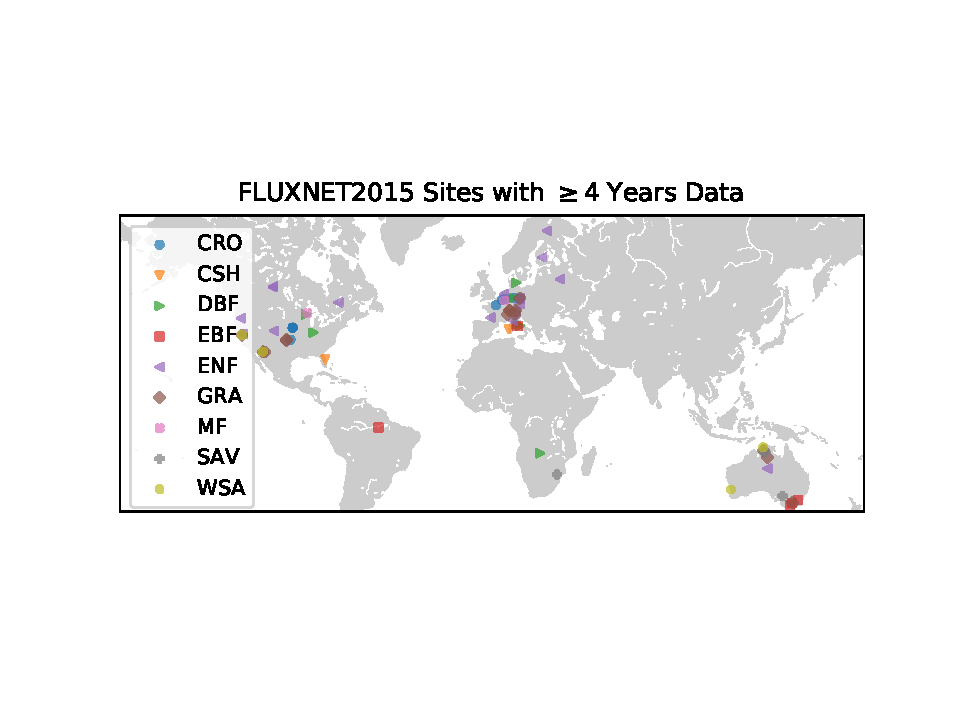
\includegraphics[trim={0 3cm 0 3cm}, clip]{./map.pdf}
  \caption{Plant functional type and location of FLUXNET2015 sites
    used in this analysis.}
  \label{map_fig}
\end{figure}

\begin{table}
  \caption{Metadata and citations for flux sites used in this analysis. All data are gathered from \url{www.fluxdata.org} using tools available at \url{https://github.com/trevorkeenan/FLUXNET_citations}.}
  \label{flux_sites}
  \label{definitions}
  \centering \footnotesize
  \begin{tabular}{l l l l l l l}
    \hline
    Site name & PFT & Lat & Lon & Clim$^{a}$ & Period & References \\
    \hline
    AT-Neu & GRA & 47.1167 & 11.3175 & Unk & 2002-2012 & \cite{AT-Neu} \\
AU-ASM & ENF & -22.2830 & 133.2490 & Unk & 2010-2013 & \cite{AU-ASM} \\
AU-Cpr & SAV & -34.0021 & 140.5891 & Unk & 2010-2014 & \cite{AU-Cpr} \\
AU-DaP & GRA & -14.0633 & 131.3181 & Aw  & 2007-2013 & \cite{AU-DaP} \\
AU-DaS & SAV & -14.1593 & 131.3881 & Aw  & 2008-2014 & \cite{AU-DaS} \\
AU-Dry & SAV & -15.2588 & 132.3706 & Unk & 2008-2014 & \cite{AU-Dry} \\
AU-Gin & WSA & -31.3764 & 115.7138 & Unk & 2011-2014 & \cite{AU-Gin} \\
AU-How & WSA & -12.4943 & 131.1523 & Aw  & 2001-2014 & \cite{AU-How} \\
AU-Rig & GRA & -36.6499 & 145.5759 & Unk & 2011-2014 & \cite{AU-Gin} \\
AU-Stp & GRA & -17.1507 & 133.3502 & Unk & 2008-2014 & \cite{AU-DaP} \\
AU-Tum & EBF & -35.6566 & 148.1517 & Cfb & 2001-2014 & \cite{AU-Tum} \\
AU-Whr & EBF & -36.6732 & 145.0294 & Unk & 2011-2014 & \cite{AU-Whr} \\
AU-Wom & EBF & -37.4222 & 144.0944 & Unk & 2010-2012 & \cite{AU-Wom} \\
BE-Lon & CRO & 50.5516 & 4.7461 & Cfb & 2004-2014 & \cite{BE-Lon} \\
BE-Vie & MF & 50.3051 & 5.9981 & Cfb & 1996-2014 & \cite{BE-Vie} \\
BR-Sa3 & EBF & -3.0180 & -54.9714 & Am & 2000-2004 & \cite{BR-Sa3} \\
CA-Qfo & ENF & 49.6925 & -74.3421 & Dfc & 2003-2010 & \cite{CA-Qfo} \\
CA-SF1 & ENF & 54.4850 & -105.8176 & Dfc & 2003-2006 & \cite{CA-SF1} \\
CA-SF2 & ENF & 54.2539 & -105.8775 & Dfc & 2001-2005 & \cite{CA-SF1} \\
CH-Cha & GRA & 47.2102 & 8.4104 & Unk & 2005-2014 & \cite{CH-Cha} \\
CH-Dav & ENF & 46.8153 & 9.8559 & Unk & 1997-2014 & \cite{CH-Dav} \\
CH-Fru & GRA & 47.1158 & 8.5378 & Unk & 2005-2014 & \cite{CH-Fru} \\
DE-Geb & CRO & 51.1001 & 10.9143 & Unk & 2001-2014 & \cite{DE-Geb} \\
DE-Gri & GRA & 50.9500 & 13.5126 & Cfb & 2004-2014 & \cite{DE-Gri} \\
DE-Hai & DBF & 51.0792 & 10.4530 & Unk & 2000-2012 & \cite{DE-Hai} \\
DE-Kli & CRO & 50.8931 & 13.5224 & Cfb & 2004-2014 & \cite{DE-Gri} \\
DE-Lkb & ENF & 49.0996 & 13.3047 & Unk & 2009-2013 & \cite{DE-Lkb} \\
DE-Obe & ENF & 50.7867 & 13.7213 & Cfb & 2008-2014 & {\textendash} \\
DE-Seh & CRO & 50.8706 & 6.4497 & Unk & 2007-2010 & \cite{DE-Seh} \\
DE-Tha & ENF & 50.9624 & 13.5652 & Cfb & 1996-2014 & \cite{DE-Tha} \\
DK-Sor & DBF & 55.4859 & 11.6446 & Unk & 1996-2014 & \cite{DK-Sor} \\
FI-Hyy & ENF & 61.8474 & 24.2948 & Unk & 1996-2014 & \cite{FI-Hyy} \\
FI-Sod & ENF & 67.3619 & 26.6378 & Unk & 2001-2014 & \cite{FI-Sod} \\
FR-Gri & CRO & 48.8442 & 1.9519 & Cfb & 2004-2013 & \cite{FR-Gri} \\
FR-LBr & ENF & 44.7171 & -0.7693 & Unk & 1996-2008 & \cite{FR-LBr} \\
IT-Col & DBF & 41.8494 & 13.5881 & Unk & 1996-2014 & \cite{IT-Col} \\
IT-Cpz & EBF & 41.7052 & 12.3761 & Unk & 1997-2009 & \cite{IT-Cpz} \\
IT-Lav & ENF & 45.9562 & 11.2813 & Unk & 2003-2014 & \cite{IT-Lav} \\
IT-MBo & GRA & 46.0147 & 11.0458 & Unk & 2003-2013 & \cite{IT-MBo} \\
IT-Noe & CSH & 40.6061 & 8.1515 & Unk & 2004-2014 & \cite{IT-Noe} \\
IT-Ren & ENF & 46.5869 & 11.4337 & Unk & 1998-2013 & \cite{IT-Ren} \\
IT-Ro2 & DBF & 42.3903 & 11.9209 & Unk & 2002-2012 & \cite{IT-Ro2} \\
IT-SRo & ENF & 43.7279 & 10.2844 & Unk & 1999-2012 & \cite{IT-SRo} \\
IT-Tor & GRA & 45.8444 & 7.5781 & Unk & 2008-2014 & \cite{IT-Tor} \\
NL-Loo & ENF & 52.1666 & 5.7436 & Unk & 1996-2013 & \cite{NL-Loo} \\
RU-Fyo & ENF & 56.4615 & 32.9221 & Unk & 1998-2014 & \cite{RU-Fyo} \\
US-AR1 & GRA & 36.4267 & -99.4200 & Dsa & 2009-2012 & \cite{US-AR1} \\
US-AR2 & GRA & 36.6358 & -99.5975 & Dsa & 2009-2012 & \cite{US-AR1} \\
US-ARM & CRO & 36.6058 & -97.4888 & Cfa & 2003-2012 & \cite{US-ARM} \\
US-Blo & ENF & 38.8953 & -120.6328 & Csa & 1997-2007 & \cite{US-Blo} \\
US-KS2 & CSH & 28.6086 & -80.6715 & Cwa & 2003-2006 & \cite{US-KS2} \\
US-MMS & DBF & 39.3232 & -86.4131 & Cfa & 1999-2014 & \cite{US-MMS} \\
US-Me2 & ENF & 44.4523 & -121.5574 & Csb & 2002-2014 & \cite{US-Me2} \\
US-NR1 & ENF & 40.0329 & -105.5464 & Dfc & 1998-2014 & \cite{US-NR1} \\
US-Ne1 & CRO & 41.1651 & -96.4766 & Dfa & 2001-2013 & \cite{US-Ne1} \\
US-Ne2 & CRO & 41.1649 & -96.4701 & Dfa & 2001-2013 & \cite{US-Ne1} \\
US-Ne3 & CRO & 41.1797 & -96.4397 & Dfa & 2001-2013 & \cite{US-Ne1} \\
US-SRG & GRA & 31.7894 & -110.8277 & Bsk & 2008-2014 & \cite{US-SRG} \\
US-SRM & WSA & 31.8214 & -110.8661 & Bsk & 2004-2014 & \cite{US-SRM} \\
US-Syv & MF & 46.2420 & -89.3477 & Dfb & 2001-2014 & \cite{US-Syv} \\
US-Ton & WSA & 38.4316 & -120.9660 & Csa & 2001-2014 & \cite{US-Ton} \\
US-Var & GRA & 38.4133 & -120.9507 & Csa & 2000-2014 & \cite{US-Var} \\
US-WCr & DBF & 45.8059 & -90.0799 & Dfb & 1999-2014 & \cite{US-WCr} \\
US-Wkg & GRA & 31.7365 & -109.9419 & Bsk & 2004-2014 & \cite{US-Wkg} \\
ZA-Kru & SAV & -25.0197 & 31.4969 & Unk & 2000-2010 & \cite{ZA-Kru} \\
ZM-Mon & DBF & -15.4378 & 23.2528 & Unk & 2000-2009 & \cite{ZM-Mon} \\

    \hline
    \multicolumn{7}{l}{$^{a}$K{\"o}ppen Climate classification.}
    \hline
\end{table}



The purpose of this study is to examine ecosystem response to
atmospheric drying, focusing on the growing season. To accomplish
this, we filter and quality control the data using a similar procedure
as \cite{Zhou_2015}:
\begin{itemize}
\item Only measured or highest (``good'') quality gapfilled data,
  according to quality control flags, are used.
\item To isolate the growing season, we only use days in which the
  average Gross Primary Productivity (GPP) exceeds 10\% of the
  observed 95th percentile of GPP for a given site. GPP is calculated
  using the nighttime respiration partitioning method.
\item We remove days with rain and the day following to avoid issues
  with rain interception and sensor saturation at high relative
  humidity (\cite{Medlyn_2017}).
\end{itemize}
Additionally, as in \citet{Lin_2018}, we restrict data to the daytime,
which is identified when downwelling shortwave radiation is greater
than 50 W m$^{-2}$ and sensible heat flux is greater than 5 W
m$^{-2}$. To reduce the chance of sensor saturation at high relative
humidity, we remove all time steps for which VPD is less than .01 kPa,
and to reduce errors at low windspeeds we remove all periods with wind
magnitudes less than 0.5 m s$^{-1}$. Timesteps with negative observed
GPP or ET are also removed, and we aggregate half hourly data to
hourly averages to reduce noise \citep{Lin_2018}. After these quality
control procedures, 434,765 upscaled hourly observations remain.

\subsection{Methods}
\label{methods}
The Penman-Monteith equation \citep [hereafter PM,][]{Penman_1948,
  Monteith_1965} estimates ET as a function of observable atmospheric
variables and surface conductances:
% \begin{linenomath*}
  \begin{equation}
    \label{orig_pen}
    ET = \frac{\Delta R_{net} + g_a \rho_a c_p VPD}{\Delta + \gamma(1 + \frac{g_a}{g_s})},
  \end{equation}
% \end{linenomath*}
where $\Delta$ is the change in saturation vapor pressure with
temperature, given by Clausius-Clapeyron ($\frac{d \; e_s}{d \; T}$),
$R_{net}$ is the net radiation minus ground heat flux, $g_a$ is
aerodynamic conductance, $\rho_a$ is air density, $c_p$ is specific
heat of air at constant pressure, $\gamma$ is the psychometric
constant, and $g_s$ is the stomatal conductance (Table
\ref{definitions}).

\begin{table}
  \caption{Definition of symbols and variables, with citation for how
    values are calculated, if applicable.}
  \label{definitions}
  \centering \footnotesize
  \begin{tabular}{l c c c}
    \hline
    Variable & Description & Units & Citation \\
    \hline
    $e_s$  & saturation vapor pressure & Pa  & - \\ 
    $T$  & temperature  & K & - \\
    $P$  & pressure & Pa  & - \\
    $\Delta$  & $\frac{\partial e_s}{\partial T}$ & Pa K$^{-1}$ & - \\
    $R_{net}$  & net radiation at land surface minus ground heat flux & W m$^{-2}$   & - \\
    $g_a$  & aerodynamic conductance & m s$^{-1}$  & \citet{Shuttleworth_2012} \\
    $\rho_a$  & air density & kg m$^{-3}$  & - \\
    $c_p$  & specific heat capacity of air at constant pressure & J K$^{-1}$ kg$^{-1}$ & - \\
    $VPD$  & vapor pressure deficit & Pa  & - \\
    $\gamma$  & psychometric constant & Pa K$^{-1}$   & - \\
    $g_{s-leaf}$  & leaf-scale stomatal conductance & m s$^{-1}$  & \citet{MEDLYN_2011} \\
    $g_{s}$  &  stomatal conductance & m s$^{-1}$
                                   & \citet{Medlyn_2017} \\
    $g_{1-leaf}$  & leaf-scale slope parameter & Pa$^{0.5}$
                                   & \citet{MEDLYN_2011} \\
    $g_{1}$  & ecosystem-scale slope parameter & Pa$^{0.5}$ & \citet{Medlyn_2017} \\
    $R$ & universal gas constant & J mol$^{-1}$ K$^{-1}$ & - \\
    $R_{air}$ & gas constant of air & J  K$^{-1}$ kg$^{-1}$ & - \\
    $\sigma$ & uncertainty parameter & -& - \\
    $c_a$ & CO$_2$ concentration & $\mu$ mol CO$_2$ mol$^{-1}$ air& - \\
    $\lambda$ & marginal water cost of leaf carbon & mol H$_2$O mol$^{-1}$ CO$_2$ & - \\
    $\Gamma$ & CO$_2$ compensation point & - & - \\
    $\Gamma^*$ & CO$_2$ compensation point without dark respiration & - & - \\
    \hline
  \end{tabular}
\end{table}


\citet{MEDLYN_2011} developed a model for stomatal conductance ($g_s$)
by combining an optimal photosynthesis theory \citep{Cowan_1977} with an empirical approach, which describes the
dependence of $g_s$ to VPD. This resulted in the following model for
leaf-scale stomatal conductance:

% \begin{linenomath*}
  \begin{equation}
    g_{s-leaf} = g_0 + 1.6 \left(1 +
      \frac{g_{1-leaf}}{\sqrt{VPD}}\right) \frac{A}{c_a},
    \label{leaf_medlyn}
  \end{equation}
% \end{linenomath*}
where $g_{1-leaf}$ is a leaf-scale ``slope'' parameter, A is the net
CO$_2$ assimilation rate, and $c_a$ is the atmospheric CO$_2$
concentration at the leaf surface. \cite{MEDLYN_2011} relate the slope
parameter ($g_{1-leaf}$) to physical parameters as:
% \begin{linenomath*}
  \label{slope}
  \begin{equation}
    g_{1-leaf} = \sqrt{\frac{3 \, \Gamma^* \, \lambda}{1.6}},\footnote{Note this expression has units of of (mmol mol$^{-1}$)$^{1/2}$, but this can be converted to Pa$^{1/2}$ using the ideal gas law.}
  \end{equation}
% \end{linenomath*}

where $\Gamma^*$ is the CO$_2$ compensation point for photosynthesis
(without dark respiration), and $\lambda$ is the marginal water cost
of leaf carbon
($\frac{\partial \; \text{transpiration}}{\partial \; A}$). So,
$g_{1-leaf}$ is a leaf-scale term reflecting the trade-off of water for
carbon uptake. The higher $g_{1-leaf}$, the more open the stomata and
the more they release water in exchange for carbon.


The Medlyn model for stomatal conductance has been shown to behave
very well across PFTs \citep[][]{Lin_2015}, and has been successfully
adopted to ecosystem scale analysis in \citet{Medlyn_2017}. In units
of m s$^{-1}$, the ecosystem scale stomatal conductance is:

% \begin{linenomath*}
  \begin{equation}
    g_s = \frac{R \,T}{P} \; 1.6 \left(1 + \frac{g_1}{\sqrt{VPD}}\right) \frac{GPP}{c_a},
    \label{medlyn}
  \end{equation}
% \end{linenomath*}

where GPP is the ecosystem scale gross primary production, and $g_1$
is an ecosystem scale analogue to $g_{1-leaf}$. We solve for $g_1$
following \citet{Medlyn_2017} (Equation 5), and take the median $g_1$
value to be representative of each PFT (Table \ref{pft}) instead of the mean to avoid extra weighting of rare outliers.

\begin{table}
  \caption{Plant functional types, their abbreviation, calculated
    Medlyn coefficient, and calculated uWUE. uWUE from
    \citet{Zhou_2015}, including the observed standard deviation, is
    shown for comparison. Note that uWUE from \citet{Zhou_2015} is
    calculated from a different set of sites, and that units are
    converted such that the quantities work with Equations 1-8 and the
    variables defined Table \ref{definitions}.}
  \small
  \label{pft}
  \centering
  \begin{tabular}{l c c @{\qquad} c c}
    \hline
    \multirow{2}[3]{*}{Abbreviation} & \multirow{2}[3]{*}{PFT} & \multirow{2}[3]{*}{$g_1$ (Pa$^{0.5}$)} & \multicolumn{2}{c}{uWUE ($\mu$-mol [C] Pa$^{0.5}$ J$^{-1}$ [ET])}  \\
    \cmidrule{4-5}

                                     & & & fitted & \citet{Zhou_2015} \\

    \hline
    \input{pft_params.tex}
    \hline
  \end{tabular}
\end{table}

While Equation 3 can be used in PM (Equation 1), it will make
analytical work with the function intractable because $GPP$ is
functionally related to ET itself. Additionally, a perturbation to VPD
should induce a physiological plant response that will alter GPP and
cause an indirect change in stomatal conductance, in addition to the
direct effect of VPD in Equation \ref{medlyn}. Therefore, in order to
derive the response of ET to VPD, we must account for the functional
relationship between GPP, ET, and VPD, and its effect on stomatal
conductance. We can use aforementioned semi-empirical results of
\citet{Zhou_2015} as a tool to approach this
problem. \citet{Zhou_2015}, showed that  underlying Water Use
Efficiency (uWUE):

% \begin{linenomath*}
  \begin{equation}
    uWUE = \frac{GPP \cdot \sqrt{VPD}}{ET}
    \label{uwue}
  \end{equation}
% \end{linenomath*}

is relatively constant across time and moisture conditions within a
plant functional type, and correctly captures a constant relationship
between GPP, ET and VPD over a diurnal cycle \citep{Zhou_2014}. The
theoretical derivation of the square root VPD dependence in $uWUE$
leverages the same assumptions used in \cite{MEDLYN_2011} to derive the
square-root VPD dependence of the stomatal conductance model (Equation
\ref{medlyn}).  We can use uWUE to remove the $GPP$ dependence from
$g_s$ in a way that makes PM analytically tractable:

% \begin{linenomath*}
  \begin{equation}
    g_s = \frac{R \, T}{P} 1.6 \left(1 + \frac{g_1}{\sqrt{VPD}}\right) \frac{uWUE \; ET}{c_a \; \sqrt{VPD}}.
    \label{new_g_s}
  \end{equation}
% \end{linenomath*}

Plugging Equation \ref{new_g_s} into Equation \ref{orig_pen} and
rearranging gives a new explicit expression for PM, in which
dependence on $GPP$ is removed:

% \begin{linenomath*}
  \begin{equation}
    ET = \frac{\Delta R_{net} + \frac{g_a\; P}{T} \left( \frac{ c_p VPD}{R_{air}} -  \frac{\gamma c_a \sqrt{VPD} }{ R \; 1.6\; \text{ uWUE } (1 + \frac{g_1}{\sqrt{VPD}})} \right) }{ \Delta + \gamma}
    \label{et}
  \end{equation}
% \end{linenomath*}

By accounting for photosynthesis changes in ecosystem conductance, with
Equation \ref{et} we have derived for the first time, using recent
results \citep[][]{MEDLYN_2011, Zhou_2014, Zhou_2015, Medlyn_2017}, ET
explicitly as function of environmental variables and two
plant-specific constants, the slope parameter ($g_1$), and uWUE, both
reflecting water conservation strategy. The slope parameter is related
to the willingness of stomata to trade water for CO$_2$ and to keep
stomata open. uWUE is a semi-empirical ecosystem-scale constant
related to how WUE changes with VPD (specifically $VPD^{-1/2}$). It is
also roughly proportional to physical constants:

\[uWUE \appropto \sqrt{\frac{c_a - \Gamma}{1.6 \lambda}},\]

where $\Gamma$ is the CO$_2$ compensation point \citep[Equation 5
in][]{Zhou_2014}. So uWUE is related to atmospheric CO$_2$
concentration and compensation point, and is inversely proportional to
the marginal water cost of leaf carbon.

Given eddy-covariance FLUXNET2015 data (Section \ref{data}), every
term in our new version of PM (Equation \ref{et}) is observed, except
for uWUE, which we fit by calculating its expectation, given the model
and FLUXNET2015 data.

However, eddy-covariance data are inherently noisy so we include a
measure of uncertainty in our analysis. To account for observational
error, as well as model uncertainty (e.g. temporal and spatial
variations of uWUE and $g_1$), we introduce an uncertainty parameter
$\sigma$ modifying uWUE:

% \begin{linenomath*}
  \begin{equation}
    ET = \frac{\Delta R_{net} + \frac{g_a\; P}{T} \left( \frac{ c_p VPD}{R_{air}} -  \frac{\gamma c_a \sqrt{VPD} }{ R \; 1.6\; \sigma \; \text{ uWUE } (1 + \frac{g_1}{\sqrt{VPD}})} \right) }{ \Delta + \gamma}
    \label{et_sigma}
  \end{equation}
% \end{linenomath*}

Now, from each FLUXNET2015 observation (i.e. for each hourly
observation at every time step) we can evaluate $\sigma$:

% \begin{linenomath*}
  \begin{equation}
    \sigma = - \frac{g_a \gamma c_a \sqrt{VPD} L_v P }{ \left(\text{ ET } ( \Delta + \gamma) - \Delta R_{net} - g_a \rho_a c_p VPD\right) 1.6 \; R\; T\; \text{ uWUE } (1 + \frac{g_1}{\sqrt{VPD}})},
    \label{sigma}
  \end{equation}
% \end{linenomath*}

Thus, with this uncertainty analysis we can evaluate departure from
our theory in observations, as a departure of $\sigma$ from unity. The
variability of $\sigma$ across sites and time provides a measure of
uncertainty in our model, assumptions, as well as in the FLUXNET2015
observations themselves. The variability of $\sigma$ then propagates
through any uncertainty to our partial derivative of Equation
\ref{et_sigma} with respect to VPD:

% \begin{linenomath*}
  \begin{equation}
    \frac{\partial \;  ET}{\partial \; VPD} = \frac{2\; g_a \; P}{T(\Delta + \gamma)}   \left(\frac{ c_p}{R_{air}} -  \frac{\gamma c_a }{1.6 \; R\; \sigma \; \text{ uWUE }} \left( \frac{2 g_1 + \sqrt{VPD}}{2 (g_1 + \sqrt{VPD})^2}\right) \right)
    \label{d_et}
  \end{equation}
% \end{linenomath*}

With Equation \ref{d_et} we have an analytical framework for ecosystem
response to atmospheric demand perturbations with environmental
conditions held fixed. There are a few subtleties to taking the
derivative in Equation \ref{d_et}: $\Delta$ ($\frac{d e_{s}}{d T}$)
and $VPD$ are functionally related, so while taking the derivative we
evaluate
$\frac{\partial \; ET}{\partial \; VPD} = \frac{\partial \; ET}
{\partial \; e_s} \frac{\partial \; e_s}{\partial \; VPD}
\Big|_{\text{RH fixed}} + \frac{\partial \; ET}{\partial \; RH}
\frac{\partial \; RH}{\partial \; VPD} \Big|_{\text{$e_s$
    fixed}}$. $RH$ and $e_s$ are assumed to be approximately
independent, which is supported by the data (not shown).

This derivation relied either implicitly or explicitly on several
assumptions. First, we assume that VPD at the leaf surface is the same
as VPD at measurement height; physically this implies that leaves are
perfectly coupled to the atmosphere. In reality, for some conditions
and plant types the leaves can become decoupled from the boundary
layer \citep{De_2017, Medlyn_2017}. Given our focus on the growing
season, which is usually characterized by relatively high insolation
inducing instability and convective boundary layers, we would expect
the surface to be generally well coupled. An additional assumption in
the formulation of $uWUE$ \citep{Zhou_2014, Zhou_2015} and
\citet{Medlyn_2017}'s stomatal conductance model is that direct soil
evaporation (E) contributions to ET remain small relative to
transpiration (T). This should be more true during the growing
season. The ratio of E to T may increase immediately after rainfall
events due to high soil moisture and ponding, but VPD is generally low
anyways during these times. However, some plant types allow for
systematically larger contributions of E in ET, particularly those
with sparse canopies and smaller relative amounts of transpiration. We
therefore might expect that the theory will be most applicable to
forest PFTs, which will be most strongly coupled to the boundary layer
due to larger surface roughness, and will also generally have the
highest ratios of transpiration to evaporation. Finally, for the goal
of developing PFT-wide intuition, we assume that $g_1$ and $uWUE$ are
constant in space and time. Both quantities have been shown to be well
conserved over space and time within a PFT relative to inter-PFT
variability. However, we would expect them to vary somewhat with
environmental conditions including very low soil water content,
temperature, and with intra-PFT plant-specific characteristics like
wood density for tree PFTs \citep{Lin_2015}. Given these strong
assumptions made with the goal of understanding broad, leading order
plant behaviors, we take the extra care of including and analyzing
uncertainty (Section \ref{testing}) and examining sensitivity to the
exponent of the VPD response (Section \ref{functional_form}).

We note one final comment on our derivation which is relevant for
drought indices. If we approximate $c_a$ at a global mean CO$_2$
concentration, then the RHS of Equation \ref{et} is fully defined
using commonly available weather station data and the constants
published here. This makes Equation \ref{et} a useful alternative to
PET in drought indices and hydrometeorological analysis for vegetated
surfaces. Equation \ref{et} better reflects the physics of water
exchange at the land surface and would only require fitting of uWUE
and $g_1$, and can also account for changes in CO$_2$ concentration
(assuming some relationship between $\lambda$ and [CO$_2$]), contrary
to typical drought indices such as the Palmer Drought Severity Index
(PDSI) \citep{Swann_2016, Lemordant_2016, Lemordant_2018}. Lastly, all
code and data used in this analysis, including those used to generate
the figures and tables, are publicly available at
\url{https://github.com/massma/climate\_et}.
%\hyperref[https://github.com/massma/climate\_et]{https://github.com/massma/climate_et}.

\section{Results and Discussion}
\label{results}

By construction, the variability in the $\sigma$ term (Equation
\ref{sigma}) contains all model and observational uncertainties. For
an observation that perfectly matches our model and constant uWUE
assumption, $\sigma$ will be one. Therefore, for our assumptions and
framework to be reasonable $\sigma$ should be close to 1. An
additional concern is that $\sigma$ may in fact be correlated with
$VPD$, in which case the dependence would need to be accounted for
when taking the derivative. Fortunately, there is a very weak
dependence of $\sigma$ on VPD in their joint distribution, and
$\sigma$ is indeed close to unity i.e. $O(1)$ (Figure
\ref{joint_vpd_sigma}). Given this weak dependence and the
distribution of $\sigma$ we have confidence in our model framework and
the data quality.

\begin{figure}[h]
  \centering\includegraphics[width=0.75\textwidth]{./joint_vpd_sigma.pdf}
  \caption{The joint distribution of $VPD$ and $\sigma$, with outliers
    removed (defined as lowest and highest 5\% of $\sigma$). $\sigma$
    exhibits a weak dependence on $VPD$, and $\sigma$ is $O(1)$ for
    the bulk of the observations.}
  \label{joint_vpd_sigma}
\end{figure}

Before calculating the sensitivity of ET to VPD, we will consider the
functional form of Equation \ref{d_et}. There are two main terms: a
``scaling'' term, which modifies the magnitude but not the sign of the
ET response to VPD ($\frac{\partial \; ET}{\partial \; VPD}$):

\begin{equation}
  \frac{g_a \; P}{T(\Delta + \gamma)},
\end{equation}

and a ``sign'' term, which determines whether ET increases or
decreases with VPD (i.e. atmospheric demand driven or physiologically
controlled):

\begin{equation}
  \label{sign}
  \frac{c_p}{R_{air}} - \frac{\gamma c_a }{1.6 \; R\; \text{ uWUE }} \left( \frac{2 g_1 + \sqrt{VPD}}{2 (g_1 + \sqrt{VPD})^2}\right).
\end{equation}
All variables are positive, so the relative magnitude between the
first term and the second term in the sign term (Equation \ref{sign})
will determine whether ET increases or decreases with increasing
VPD. If the second term is larger then plant control dominates and ET
decreases with increasing VPD. However, if the first term is larger,
then atmospheric demand dominates and ET increases with increasing
VPD.

\subsection{Functional Form of the Sign Term}
\label{sign_term}
First, we explore the variables within the sign term to gain better
intuition on the driver of either the increase or reduction of ET with
VPD. CO$_2$ concentration ($c_a$) and the psychometric constant
($\gamma$) are relatively constant over the dataset considered here so
that the variability is dominated by $\sigma$ and $VPD$. uWUE could
vary with soil moisture but has been shown to be relatively constant
\citep{Zhou_2015}. This then means that the sign term only depends on
VPD for a given PFT and is approximately just a function of $VPD$. We
can further determine a critical threshold separating an increase from
a decrease in ET, i.e. the threshold $VPD_{crit}$ such that the
derivative vanishes $\frac{\partial \; ET}{\partial \; VPD} = 0$:
\small
% \begin{linenomath*}
  \begin{equation}
    VPD_{crit} = \frac{R_{air}}{4 c_p} \left( \frac{\gamma c_a}{1.6\; R \;  uWUE} + \sqrt{\frac{\gamma c_a}{1.6\; R \;  uWUE}\left( \frac{\gamma c_a}{1.6\; R \;  uWUE} + 8 g_1 \frac{c_p}{R_{air}}\right)} - 4 g_1 \frac{c_p}{R_{air}} \right),
    \label{vpd_min_et}
  \end{equation}
% \end{linenomath*}
\normalsize noting that $VPD_{crit}$ mostly depends on the PFT
parameters uWUE and $g_1$, and only varies weakly with climate as most
other parameters related to the environment are nearly constant. The
calculated value of $VPD_{crit}$ for each PFT is shown in Table
\ref{vpd_crit}. For any values of $VPD$ less than $VPD_{crit}$, ET
will decrease with increasing VPD
($\frac{\partial \; ET}{\partial \; VPD} < 0$), and for values of
$VPD$ greater than $VPD_{crit}$, ET will increase with increasing VPD
($\frac{\partial \; ET}{\partial \; VPD} > 0$). In other words,
ecosystems regulate and mitigate evaporative losses up to the VPD
limit, $VPD_{crit}$, above which atmospheric demand is just too high
to be entirely compensated by stomatal and ecosystem regulation. We
note however that even though ET increases again above the critical
threshold, $VPD_{crit}$, ET is still much lower than potential
evaporation as stomata are still strongly regulating vapor fluxes to
the atmosphere. Indeed, even in the absence of soil pore evaporation,
stomata do not shut down entirely at very high VPD so that ET does not
go to zero, because stomata are still slightly open to perform some
photosynthesis \citep{Ball_1987, Leuning_1990, MEDLYN_2011}. In
addition, upward xylem transport is necessary to maintain phloem
transport, as well as nutrient transport and thus carbon allocation
\citep{De_2013, Nikinmaa_2013, Ryan_2014}.

\begin{table}
  \caption{Values of $VPD_{crit}$, where
    $\frac{\partial \; ET}{\partial \; VPD} = 0$, evaluated at PFT
    average values for $R_{air}$, $\gamma$, and $c_a$. PFT-specific
    constants ($g_1$, uWUE) are provided in Table \ref{pft}. For
    values of $VPD$ less than $VPD_{crit}$,
    $\frac{\partial \; ET}{\partial \; VPD}$ will be negative, and for
    values of $VPD$ greater than $VPD_{crit}$,
    $\frac{\partial \; ET}{\partial \; VPD}$ will be positive.}
  \centering
  \begin{tabular}{l c c c c c}
    \hline
    PFT & $R_{air}$ & $c_a$ (ppm) & $\gamma$  & \textbf{$VPD_{crit}$ (Pa)} \\
    \hline
    \input{vpd_crit.tex}
    \hline
  \end{tabular}
  \label{vpd_crit}
\end{table}


Differences in $VPD_{crit}$ are exclusively determined by uWUE and the
slope parameter ($g_1$) related to the plant functional type. A larger
uWUE means a smaller $VPD_{crit}$, and an ET response to increases VPD
that is more likely to be positive. At first glance this result is
somewhat counter-intuitive; we expect that plants with a higher water
use efficiency would be more water conservative. However, in reality
uWUE determines how $WUE$ changes with VPD:

\[WUE = \frac{GPP}{ET} = \frac{uWUE}{\sqrt{VPD}}.\]
\[\frac{\partial \; WUE}{\partial \; VPD} = -\frac{uWUE}{2 \;
    VPD^{3/2}}\]

So, plants with a higher uWUE will have a greater \textit{decrease} in
ecosystem-scale $WUE$ in response to increases in VPD. This decrease
in $WUE$ causes more water loss per unit carbon gain, and explains the
relationship between high uWUE and high likelihood of increases of ET
in response to increasing atmospheric drying (increases in VPD).

A tendency towards increasing ET response with increasing VPD can also
be caused by a high slope parameter ($g_1$), characteristic of plants
that at the leaf scale are more willing to trade water for access to
atmospheric CO$_2$. Plants that are less conservative will be thus be
more likely to increase ET with increasing VPD. Both the
aforementioned effects (large uWUE, $g_1$) can amplify each other, and
generally conspire to shift the sign term towards a positive value for
a given PFT.

This effect of uWUE and $g1$ on the sign term is most apparent by
comparing two extreme PFTs: water intensive crops (CRO) and water
conservative closed shrub (CSH). CRO has higher slope parameter and a
slightly higher uWUE ($g_1 = 140.7$ Pa$^{1/2}$; $2.85$ $\mu$-mol [C]
Pa$^{0.5}$ J$^{-1}$ [ET]) compared to CSH ($g1 = 75.1 \, Pa^{1/2}$,
$uWUE=2.82$ $\mu$-mol [C] Pa$^{0.5}$ J$^{-1}$ [ET]). These differences
in PFT parameters cause opposite ET responses to changes in VPD
between CRO and CSH. ET theoretically always decreases with increasing
VPD for the more water conservative CSH, while ET frequently increases
with increasing VPD for the more water intensive CRO (Figure
\ref{idealized_sign}). CROs evolved or were bred to prioritize GPP and
yield and are thus not water conservative. They are very willing to
trade water for photosynthesis and productivity, despite changes in
VPD, while CSH are very unwilling to trade water for more
photosynthesis.

\begin{figure}
  \centering \includegraphics{./idealized_sign.pdf}
  \caption{The functional form of the sign term, with $\sigma$ held
    fixed at 1, and all terms except VPD set to PFT averages. For
    comparison, the observed range of VPD for each PFT is plotted
    below the x-axis. Stars denote 25th, 50th, and 75th percentiles,
    and the range of the line spans the 5th-95th percentiles of
    observed VPD. Vertical black lines denote the location of
    $VPD_{crit}$ for each PFT, with the exception of CSH and WSA, for which
    $VPD_{crit}$ is off-scale.}
  \label{idealized_sign}
\end{figure}


As expected, the slope parameter ($g_1$) is a primary determinant of
the VPD dependence for the sign term shown in Figure
\ref{idealized_sign}. Plants that are more conservative (small $g_1$)
will tend to reduce ET with increasing VPD, and will be very effective
at reducing ET, especially at low VPD. However, at very high VPD,
gradients in vapor pressure at the leaf scale will become very strong
as stomata reach their limits of closure in response to VPD
(parameterized with $g_1$). As a result, ET response will begin to
asymptote towards a constant ecosystem-scale values as leaf-scale
response to VPD asymptotes towards zero.  Therefore, plants with a low
$g_1$ will have the largest VPD dependence of ET response because the
difference in ET response at low VPD (leaf stomatal response
dominates) and high VPD (VPD gradient dominates) is largest. This is
apparent in the strong VPD dependence of CSH, which has the lowest
slope parameter ($g_1=75.1$ Pa$^{1/2}$) (Figure \ref{idealized_sign}).

To summarize our theoretical insights (Figure \ref{idealized_sign} and
Table \ref{vpd_crit}), CROs are the least water conservative and have
the strongest overall tendency to increase ET with increasing VPD,
while CSH are the most water conservative and have the strongest
tendency to decrease ET with increasing VPD, as well as the strongest
VPD dependence of response. Figure \ref{idealized_sign} clearly shows,
according to our theory, that for all PFTs except for crops there is
frequent occurrence of a negative (plant dominating) ET response to
increases in VPD. Therefore, plants are able in most atmospheric
conditions to reduce ET in response to increased VPD and thus to
reduce water loss. To better illustrate this, the ranges of observed
environmental VPDs at the FLUXNET sites are plotted parallel to the
x-axis. For CSH and WSA, VPD is always less than VPD$_{crit}$ (off scale) so
that the plant response dominates in typical environmental conditions,
emphasizing the water conservative strategy of those plants. For CRO
on the other hand, VPD is higher than VPD$_{crit}$ for more than 50\%
of observations, emphasizing that those plants operate with an
aggressive water usage strategy, are water intensive and were actually
engineered for photosynthesis rather than water saving. For DBF, EBF,
MF, GRA, and SAV more than half of the observed VPD are less than
VPD$_{crit}$, i.e. in conditions where plant response dominates. SAV
has a more water conservative response than the forest, grass, and
crop plan types, but still responds by increasing ET with increasing
VPD for about a quarter of observations, due to the high aridity (VPD)
of the SAV ecoclimate. It is also important to note that for all PFTs,
even when atmospheric demand dominates, ET response to VPD is still
far more negative than it would be for potential evaporation
$\partial PET/\partial VPD$, i.e. atmospheric demand only, emphasizing
that there is still a strong regulation of evaporative flux by stomata
and though the plant xylem. The sign term in the PET case would just
be a constant ($\frac{c_p}{R_{air}} \approx 3.5$), which is far larger
than any part of the curves for any PFT. This highlights the
deficiencies of PET's ability to capture land response to changes in
atmospheric dryness (VPD). Plants are always regulating water exchange
from the land surface, even when they reach the limits of they ability
to do so.

\subsection{Functional Form of the Scaling Term}
\label{scale_term}
While the above discussion of the sign of
$\frac{\partial \; ET}{\partial \; VPD}$ is important to answer our
question of when ET response increases or decreases with VPD,
understating the overall magnitude of the ET response is important to
soil-plant-atmosphere water budgeting. So we now more closely examine
the terms that affect how the sign term is scaled:

\begin{equation}
  \frac{g_a \; P}{T(\Delta + \gamma)}.
\end{equation}

$\frac{P}{T}$ is an air-density term, which varies little compared to
aerodynamic conductance and Clausius-Clapeyron ($\Delta$). The
psychometric constant ($\gamma$) is also relatively constant, so the
scaling term should be primarily a function of aerodynamic conductance
and temperature, through the Clausius-Clapeyron relationship
$\Delta$. This is as expected, given that the aerodynamic conductance
represents the efficiency of exchange between the surface and the
atmosphere. As aerodynamic conductance increases, any plant response
will be communicated more strongly to the atmosphere (and vice-versa).

$\Delta$'s presence in the scaling term also matches physical
intuition. $\Delta$ (and also the approximately constant $\gamma$)
control the efficiencies with which surface energy is converted to
latent and sensible heat \citep{Monteith_1965}. The functional from of
$\Delta$ will be the same across PFTs, but the temperature range may
vary slightly. In contrast, aerodynamic conductance will vary strongly
with PFT due to the importance of surface roughness for aerodynamic
conductance. So most of the differences in scaling between PFT should
be in the aerodynamic conductance term.

The control of the scaling term variability between PFTs by
aerodynamic conductance is confirmed by data (Figure
\ref{scale_vary}). Differences between PFT are almost entirely due to
differences in aerodynamic conductance, rather than differences in
observed temperature ranges. The scaling term for the tree PFTs (DBF,
EBF, ENF, MF) is generally about double the scaling terms for other
PFTs which have lower surface roughness and generally smaller
aerodynamic conductance (GRA, CSH, CRO). The savannah (WSA, SAV) PFT's
scaling is somewhere between GRA, CSH, and CRO, and DBF, EBF, ENF, and
MF, due to higher variability and surface roughness.

\begin{figure}
  % \centering
  \centerline{\includegraphics[width=1.2\textwidth]{./idealized_scale.pdf}}
  \caption{Primary sources of variability for the scaling term, as a
    function of PFT. The 5th-95th percentile range of temperature is
    plotted at the 5th, 25th, 50th, 75th, and 95th percentiles of
    aerodynamic conductance, as observed for each PFT.}
  \label{scale_vary}
\end{figure}

Within each PFT, the scaling term variability is controlled both by
environmental temperature and aerodynamic conductance variability
(Figure \ref{scale_vary}). While the observed variability of the
aerodynamic conductance contributes more to the scaling term
variability than temperature, the temperature contribution is
non-negligible. Specifically, the scaling term is generally larger at
low temperatures when latent heat is relatively inefficient at moving
energy away from the surface. This effect amplifies the role of
aerodynamic conductance variability at low temperatures.

To summarize, variability between PFTs is mostly controlled by
systematic differences in aerodynamic conductance, due to differences
in surface roughness between each PFT, and possibly to a lesser extent
wind conditions. In contrast, variability within PFT is also
controlled by temperature, through Clausius-Clapeyron. But,
aerodynamic conductance variability generally impacts the scaling term
more than temperature, even within PFTs.

\subsection{Bulk statistics of ET response to VPD}
\label{stats_sec}

In this section we consider direct observations of ET response with
eddy-covariance data, while including uncertainty with the $\sigma$
term (Section \ref{methods}). These observational results of ET
response (Table \ref{stats}) largely confirm our theoretical analysis, presented in the previous sections. For all PFTs, mean ET response to increasing VPD
is negative. However, ET response evaluated at the average of all
variables (e.g. $\sigma$, $T$, $c_a$, $VPD$) is positive for CRO, and
negative for all other PFTs. This difference in mean ET response as
compared to the ET response at mean environmental conditions is due to
the non-linear nature of the response, in which negative responses are
generally larger magnitude than positive responses (Figure
\ref{idealized_sign}). Therefore, both the mean ET response as well as
the ET response at mean environmental conditions matches our
expectations from the theory (Section \ref{sign_term}), with the
exception that CRO observations are shifted more towards a negative ET
response than we expect.

\begin{table}
  \caption{Statistics of $\frac{\partial \; ET}{\partial \; VPD}$ as a
    function of PFT.}
  \centering
  \begin{tabular}{l c c c}
    \hline
    PFT & $\overline{\frac{\partial \; ET}{\partial \; VPD}}$ & $\frac{\partial \; ET}{\partial \; VPD}\left(\overline{env}\right)$ & fraction $\frac{\partial \; ET}{\partial \; VPD} < 0.$ \\
    \hline
    \input{stats.tex}
    \hline
  \end{tabular}
  \label{stats}
\end{table}

Regarding the frequency of negative and positive ET response, all PFTs
exhibit a decreasing ET response with increasing VPD (physiologically
controlled, water conservative response) for the majority of
observations. The more water conservative PFTs generally exhibit
higher frequency of negative ET response, especially when one factors
in the distribution of environmental VPD (e.g. SAV and WSA grow in
more arid climates, Figure \ref{idealized_sign}). In general the bulk
statistics match our theoretical expectations well, with the caveat
that inclusion of uncertainty shifts crops towards a slightly more
negative response to VPD, and shifts many of the other PFTs, which still
exhibit a high frequency of negative ET response to VPD, towards more frequent
occurrence of positive ET response than the theory and Figure
\ref{idealized_sign} would suggest. The bulk statistics motivate a
more thorough examination of the structure of uncertainty and more
sophisticated validation of our theory's performance against
observations.

\subsection{Validation of theory at eddy-covariance sites}
\label{testing}
We now compare more sophisticated distributions of the observed
response to our simplified theory (Section \ref{sign_term}). The
observed distribution of the sign term, as compared to what the theory
would predict, is provided in Figure \ref{test_sign}. Our goal was to
capture the leading order behavior of the ET dependence on VPD. Given
the assumptions we made, and the uncertainties of flux tower
observations themselves, we expect a relatively large amount of noise
when reproducing the derivatives of ET. However, the data largely
reproduces our theoretical analysis.

\begin{figure}
  \centering
  \centerline{\includegraphics[width=1.2\textwidth]{./test_sign.pdf}}
  \caption{Comparison of the sign term with model uncertainty included
    (box plots) to the sign term as calculated with simplifying
    assumptions (blue line, as in Figure \ref{idealized_sign}). Each
    box plot corresponds to 5\% of the data, and the 5-95\% range of
    VPD is plotted.}
  \label{test_sign}
\end{figure}

This is particularly true for DBF and MF; the theory matches the
leading order behavior of the function when uncertainty is included,
and the observations match the theory with the addition of noise. The
VPD dependence, given by the slope parameter ($g_1$), follows the
median values of each bin. Perhaps most importantly, the x-intercept,
and thus VPD$_{crit}$, matches nearly exactly between the theory and
the observations. Therefore the sign of the ET response to increases
in VPD should be well matched, subject to the unavoidable constraints
of noise, much of which comes from the observations themselves. The
uncertainty is non negligible; there are many observations in each bin
for which the the sign of observation is opposite the response
predicted by the theory, but to leading order our theory matches the
observations well.

While CSH has a much different functional form of the sign term than
DBF and MF, CSH observations also match our theory to leading order,
albeit with a bit more variability as a function of VPD. Again, the
VPD dependence mostly determined from the slope parameter ($g_1$)
closely matches the medians in the observation bins. The
VPD-independent, strongly negative response is also captured. For CSH,
there is rare occurrence of observed positive ET response with VPD
($\approx 6$\%), even with uncertainty, so the sign of the
observations almost always matches the sign of the theory, which
states that ET response should always be negative.

Biases between the theory and observations are similar for ENF, WSA,
CRO and SAV. At low VPD the theory and the observations match
well. However, at high VPD (upper 10-20\% of observations) the theory
is biased slightly towards positive response as compared to the
observations (Figure \ref{test_sign}). For ENF this slight bias could
be explained by a negative bias in $g_1$. However, for WSA, CRO, and
SAV the observations in the highest VPD bins exhibit a downturn
towards more negative response, which cannot be captured by the
functional form of the sign term (Figure
\ref{idealized_sign}). Therefore, to explain the observations one of
the variables in the sign term must change at extreme VPD (upper
10-20\%). The most likely candidate is $uWUE$, which we have assumed
constant to meet our goal of developing intuition for leading order
behavior, but might be expected to decrease at extremely low SWC. This extremely low SWC should be correlated with high VPD in very dry environments
through sensible heating increases \citep{Gentine_2016}. The theory
for EBF exhibits similar limitations as for ENF, WSA, and SAV, except
a larger portion of observations are biased negative as compared to
the theory ($\approx$ 35\%, Figure \ref{test_sign}). However, in
general, and specifically for non-extreme VPD (VPD  $< \approx$70-90th
percentiles), the theory matches the observations for the tree and
savannah plant types well.

The theory for GRA suffers from similar, but much more severe,
limitations as for CRO, WSA, and SAV. GRA observations are
characterized by a consistent trend back towards negative ET response
at higher VPD, which the functional form of our theory is incapable of
accounting for. As compared to CRO, WSA and SAV, the divergence
between the theory and the observations is far greater for GRA,
biasing 40-50\% of observations at higher VPD. In addition for the
potential for soil moisture to alter $uWUE$, there are other sources
of plant heterogeneity specific to GRA (and some extent CRO) that may
alter $uWUE$ (or $g_1$) or invalidate other assumptions made in the
Methods section (Section \ref{methods}). We do not account for
variability in plant height and surface roughness, or differences in
C3 vs C4 photosynthesis and water strategies, which we might expect to
vary substantially across sites, years, and season for GRA. These
deficiencies could largely explain the inability of our theory to
exactly match the observations in croplands. For example, a
superposition of sites with C3 plants (at low environmental VPD) and
C4 plants (at high environmental VPD) would explain the observed shift
back towards negative ET response at high VPD when all sites are
binned together, as in Figure \ref{test_sign}. We hypothesize that the
theory would validate against observations much better if these
sources of variability were accounted for, at a cost of increased
complexity and analytical opacity. 


While the above discussion shows that our theory has some limitations
when applied to some PFTs, especially for grasslands, it does well for
DBF, MF and CSH PFTs, and captures the response at non-extreme VPD
(VPD $< \approx$ 70th-90th percentiles) for
ENF, EBF, CRO, WSA, and SAV. In general, the leading order behavior
observed in the data is captured by the theory. Departures between our
theory and observations, specifically at high VPD, could be explained
and conceptualized with shifts in $g_1$ and/or $uWUE$ due to
site-specific plant type variability (e.g. more arid-adapted ecosystems
at more arid sites), or temporal variability for some environmental
conditions (e.g. decreases in $uWUE$ at extremely low soil
moisture). To focus on general behavior and develop intuition for
PFT-scale response, we have ignored these sources of variability in
the present analysis. However, any site-specific or temporal plant
functional variability that can be conceptualized with shifts to $g_1$
and $uWUE$ can be analyzed with our framework. This opens a door to future analyses in which plant behavior in anomalous conditions
can be explained and analyzed using Equation \ref{et}.

% It is useful to also compare our theory, the observed uncertainty in
% the ET response, and PET, as PET is often used as a proxy for ET in
% hydrometeorological studies and drought indices. Again, as in our
% discussion of the theoretical results, the PET sensitivity to VPD
% will be constant at about 3.5. In Figure \ref{test_sign} the ET
% response to shifts in dryness is always far smaller than 3.5 in the
% observations, even with all uncertainty included. So the PET
% response to atmospheric dryness is outside the range of all
% observable responses. This casts doubt on PET's usefulness for
% capturing the leading order behavior of water budget and dryness
% response at the land surface, as is done in several drought
% indices. However our theory (Equation \ref{et}) could be used with
% published uWUE and $g1$ data, as an alternative to PET to estimating
% land response and dryness, and would more accurately account for the
% response to atmospheric drying.

\subsection{Observed ET response to VPD}

Most of the results presented so far focus on the sign term, so now we
turn to observations of ET response with the scaling term included
(Figure \ref{data_scatter}). Until now, in the interest of developing
leading order intuition for ET response, and to be conservative in our
acknowledgment of model and observational error, we've considered
$\sigma$ variability to be a measure of uncertainty. An alternative
viewpoint is that $\sigma \cdot uWUE$ represents spatial and temporal
variability of uWUE, which may be expected within bounds \citep[see
Table \ref{pft}, also ][]{Zhou_2015}. This is a less conservative
view; some of the $\sigma \cdot uWUE$ variability will be due to model
and observational error, so by viewing $\sigma \cdot uWUE$ as
\textit{real} variability we run the risk of mistaking noise for
signal. However, the advantage of this viewpoint is that, from
\citet{Zhou_2014}, we have very high confidence that uWUE fit at the
hourly timescale (as we do with $\sigma \cdot uWUE$) correctly
captures the relationship between ET, GPP, and VPD, and that our form
of PM introduces minimal error with its use of uWUE.

\begin{figure}
  \centering
  \centerline{\includegraphics[width=1.2\textwidth]{./data_scatter.png}}
  \caption{Scatter plots of observed
    $\frac{\partial \; ET}{\partial \; VPD}$, including $\sigma$
    variability, as a function of PFT, temperature and VPD. Please
    note differences in the colorbar scale.}
  \label{data_scatter}
\end{figure}

Therefore, with the caveat that some of the signal presented in Figure
\ref{data_scatter} may in fact be noise, we can interpret the observed
distribution of ET response to VPD. In general, the observed response
matches the intuitive theory. ET response to VPD shifts towards
positive values as VPD increases (atmospheric demand dominating). CRO
exhibit the highest occurrence of positive ET response, and the
observations confirm that CRO are the most water intensive. CSH are
the most water conservative, with a strong negative response. DBF,
EBF, ENF, MF, SAV and WSA are also water conservative, but show some
occurrence of positive ET response to VPD, particularly at higher
observed VPD, as the theory predicts. GRA, while generally water
conservative, does not match the theory well, with increasing frequency of
\textit{negative} response at high VPD. This is as expected, given
previous discussion on how we might expect more inter-site and inter-year variability for GRA (Section \ref{testing}).

Figure \ref{data_scatter} also includes the impact of the scaling
term. For a given VPD, the magnitude of ET response does not vary
strongly with temperature, confirming that any impact of the scaling
term on the magnitude of the response is primarily due to changes in
aerodynamic conductance. Intuitively this is reasonable; aerodynamic
conductance will control how dominant balances at the land surface are
communicated to the boundary layer. While $\Delta$ controls the
efficiency of energy conversion to latent heat, it appears this is a
second order term, relative to $g_a$, for scaling ET response.

As with Figure \ref{test_sign}, Figure \ref{data_scatter} matches our
expectation based on simplified theory. The sign term is most strongly
scaled by $g_a$, and in general the occurrence of positive ET response
increases as VPD increases. The willingness with which a given plant type
evolved to use water dictates the occurrence of positive versus
negative ET response. Water conservative ecosystems are highly effective
at mitigating the effects of atmospheric demand, and can store water
for later use by reducing ET in response to increasing VPD.

\subsection{Limitations of theory - very dry soil moisture conditions}
\label{swc_section}
In formulating our theory with Penman Monteith, we implicitly did not
account for very dry soil moisture conditions. For the majority of
environmental conditions observed at the eddy covariance sites used
here, soil conditions were not extremely dry so that we could assume a
constant uWUE and $g_1$. We posit that ecosystems will generally
optimize to host plants living in conditions which they evolved
for. However, in extreme conditions and drought scenarios soil water
content (SWC) could become the limiting factor for ET response to VPD,
which our theory does not account for. In addition, low soil moisture
conditions themselves increase VPD through land-atmosphere feedback
\citep[][]{Bouchet_1963, Morton_1965, Brutsaert_1999, Ozdogan_2006,
  Salvucci_2013, Gentine_2016, Berg_2016}.

Within our framework, any systematic bias due to the
failure to account for SWC's effects in very dry conditions should
manifest itself in a functional relationship between $\sigma$, our
uncertainty measure, and SWC, which is observed at the FLUXNET
sites. Examining the relationship between $\sigma$ and SWC will test
to what extent our theory breaks down in very dry soil moisture
conditions.

If we again view $\sigma \cdot uWUE$ as, in addition to a measure of
uncertainty, a short time-scale observation of uWUE, we would expect
$\sigma \cdot uWUE$ to decrease at low SWC. If $\sigma \cdot uWUE$ is
a very strong function of SWC, then our theory should be conditioned
more strongly on well watered soil conditions. If $\sigma \cdot uWUE$
is weakly a function of SWC, then our theory is more universal and
independent of soil moisture conditions.

Indeed, for all PFTs, there is some slight dependence of
$\sigma \cdot uWUE$ on SWC, especially at low SWC (Figure
\ref{swc_boxplot}). The portion of observations for which our theory
is biased by SWC-limitations varies by PFT, due to the nonlinear
threshold at which soil moisture availability limits plant
function. For CRO, MF and DBF, soil water content only matters for
about the lowest 5\% of observations (each box is 5\% of observations
in Figure \ref{swc_boxplot}). And, CRO, relative to DBF, has a very
weak dependence on soil moisture, which is reflective of the high
likelihood that CRO sites are optimally irrigated and not water
stressed, suggesting that observed departures from the theory for CRO
are due to other factors (i.e. different photosynthesis pathways; C3/C4) than soil
moisture. For ENF, EBF, SAV, and WSA, systematic SWC-induced biases in
$\sigma \cdot uWUE$ emerge in about the lowest 20-30\% of SWC
conditions, although large variability in the SWC-$(\sigma \cdot uWUE)$
relationship hampers interpretation for WSA. CSH presents a special
case: the limited number of sites (2) preclude comment on the
exact PFT-wide relationship.

In contrast to ENF, CRO, and DBF, for GRA the relationship between
$\sigma \cdot uWUE$ and SWC is more linear and affects a greater
portion of observations; about 60\% of observations. Clearly, for GRA
soil water frequently impacts plant function and alters ET response,
and our theory is limited for the majority of environmental
conditions. It is therefore not surprising that our theory tested
poorly against the data for GRA, relative to to the other PFTs
(Section \ref{testing}). For all other PFTs occurrence of soil
moisture impacts was rare enough to not manifest itself in bulk
statistics and figures.

\begin{figure}
  \centering
  \centerline{\includegraphics[width=1.2\textwidth]{./swc_boxplot.pdf}}
  \caption{$\sigma \cdot uWUE$ as a function of PFT and SWC. Each box
    plot represents 5\% of all observations. Note that the highest
    10\% of SWC observations are excluded to better resolve variability in the much more narrow bins at lower SWC (e.g. SWC has long tails at high values).}
  \label{swc_boxplot}
\end{figure}

The observed dependence of $\sigma \cdot uWUE$ on SWC for GRA would
explain the deficiencies of our theory compared to the observations in
Figure \ref{idealized_sign}, specifically the trend back towards
negative soil moisture at high VPD. Aforementioned feedbacks between
the land surface and the atmosphere, which are not accounted for due
to our focus on the one-way response of the land surface to
atmospheric conditions, would cause high VPD to be correlated with low
SWC \citep[][]{Gentine_2016, Berg_2016}. So, at high VPD observations
of low SWC are more likely, and this low SWC causes a lower uWUE
(Figure \ref{swc_boxplot}). The lower uWUE at low SWC/high VPD then
leads to the observed downturn towards decreasing ET with increasing
VPD, and the deviation between our theory (based on a constant uWUE
assumption) and observations. It is also perhaps not coincidental that
the portion of $\sigma \cdot uWUE$ affected by low soil moisture
observations is similar to the portion of observations that do not
match our theory at high VPD. Indeed, this may suggest that for all PFTs
except for GRA, coupling and feedbacks between SWC, VPD and plant
function are relatively rare. Future research will explore these relatively rare feedbacks in extreme conditions, which due to analytical intractability will require more opaque numerical analysis of many more complex processes, including boundary layer growth and state and their relationship to surface layer coupling and free-tropospheric lapse rates and humidity.

To summarize, our theory is limited by its inability to account for
soil water impacts on land surface response, and feedbacks between SWC
and VPD. Fortunately, for most PFTs SWC's effect on ET is relatively
rare ($<$30\% of observations) and does not manifest itself in the
majority of observations and bulk statistics. However for GRA, SWC decreases water use efficiency for the majority of
the observations. Soil moisture effects explain the deficiencies of
our theory in Section \ref{testing}, particularly for GRA. By
conceptualizing SWC effects as a change in $uWUE$ (and/or $g_1$), it
will be possible for future analysis to explore the importance of soil
moisture on plant response to VPD, and feedbacks between plant
function, SWC, and VPD.

\subsection{Functional form of ET dependence on VPD and its relation
  to VPD dependence}
\label{functional_form}

The theory described in Section \ref{sign_term} indicates that for a
given $uWUE$ and $g_1$, the ET dependence on VPD should be concave
upward, which is confirmed by eddy covariance data across most PFTs. In other words, there should be some local minimum in ET at a
critical VPD$_{crit}$, assuming the scaling and plant terms  (e.g. aerodynamic
conductance, $\Delta$, $g_1$ and $uWUE$) are held fixed. This result warrants further
investigation, because to our knowledge no one has derived the
theoretical ecosystem-scale relationship between ET and VPD while
controlling for other environmental conditions. In particular, from
personal communication, there is an apparent lack of consensus over
whether the shape of the ET-VPD curve should be concave upward (our
result) or concave downward in the absence of dramatic water stress. Given that understanding the ET-VPD
relationship of the one-way plant response is fundamental to
hypothesizing about any feedbacks between the land surface and the
atmosphere, we analyze why our derived ET-VPD relationship is concave
upward, particularly with respect to the exponent of VPD dependence in
$uWUE$ and the Medlyn unified stomatal conductance model.

There is a theoretical basis for the square root VPD dependence in
both the stomatal conductance model and $uWUE$ based on the assumption
that stomata behave to maximize carbon gain while minimizing water
loss, which observations also generally support \citep{Lloyd_1991,
  MEDLYN_2011, Lin_2015, Zhou_2014, Zhou_2015, Medlyn_2017}. However,
some purely empirical results that fit the exponent of the VPD
dependence to data have shown that it may vary slightly from 1/2,
suggesting that stomata, as well as ecosystem-scale quantities based
on stomata theory, may not always function optimally \citep{Zhou_2015,
  Lin_2018}. Specifically with regards to $uWUE$, one would not expect
that this ecosystem scale WUE quantity will respond to VPD exactly
analogously to stomata. Direct soil evaporation's contributions to ET
should shift the exponent of the VPD dependence, especially at
conditions of low GPP when we would expect a systematically larger
portion of direct soil evaporation contributions to ET, because we
would also expect lower amounts of transpiration at low GPP. \citet{Zhou_2015}'s
results corroborate this: they found a mean empirically fit
exponential VPD dependence of 0.55, varying slightly from the
theoretically optimal value of of 0.5 for AmeriFlux
sites. Interpreting \citet{Lin_2018}'s results, which also show
variance in the empirical exponent of the VPD dependence of the
stomatal conductance model, is more difficult as \citet{Lin_2018} do
not handle GPP/A dependence of stomatal conductance in a directly
analogous manner to the optimal theory in \citet{MEDLYN_2011} and
\citet{Medlyn_2017}. Regardless, given that these recent results on
the relationship between VPD, GPP, and ET \citep{MEDLYN_2011,
  Zhou_2014, Zhou_2015, Medlyn_2017} form the backbone of our analysis
and are what allowed us to derive an explicit ET expression for the
first time (Equation \ref{et}), we will analyze if and how assumptions
about the exponent of the VPD dependence impacts the shape of the
ET-VPD dependence. This analysis is also important to understand whether the choice of stomatal conductance model alters the fundamental behavior of the ET-VPD relationships, as many commonly used models  utilize a VPD exponent other than the 1/2 suggested by optimal theory \citep[e.g. ][ which uses an exponent of 1]{Leuning_1990}.

By introducing $n$ and $m$ we can free our stomatal
conductance model from assumptions about VPD dependence:
% \begin{linenomath*}
  \begin{equation}
    g_s = \frac{R \, T}{P} 1.6 \left(1 + \frac{g_*}{VPD^m}\right) \frac{*WUE \; ET}{c_a \; VPD^n},
    \label{m_n}
  \end{equation}
% \end{linenomath*}
where:
\[*WUE = \frac{GPP}{ET}VPD^n,\] and $g_*$ is a generic slope parameter
of units $VPD^m$. To determine how the exponent $n$ and $m$ alter the
shape of the ET-VPD dependence we find the roots of the second
derivative of ET, using Equation \ref{m_n} for stomatal conductance
($g_s$), with respect to VPD: \input{d2_solutions.tex} With this
result we have defined the family of curves separating concave up from
concave down ET solutions (Figure \ref{concave}). These curves are
only functions of the exponent of the VPD dependence and a quantity we
call non-dimensional VPD ($VPD^m/g*$). Several important
relations reveal themselves from Equation \ref{curves}:

\begin{figure}
  \centering
  \centerline{\includegraphics[width=0.75\textwidth]{./concave.pdf}}
  \caption{ Solutions corresponding to inflection points between
    concave up and concave down ET-VPD curves (Equation \ref{curves})
    for three specific scenarios. Solutions are defined in terms of a
    non-dimensional VPD ($VPD^m/g_*$), but to aide physical
    interpretation the horizontal axis is additionally provided in terms of dimensionalized VPD assuming $m=1/2$ and
    $g_*=110\; Pa^{1/2}$ (average of all PFT $g_1$). The vertical axis
    has a different interpretation depending on the solution
    curve. For the blue line ($m$ varying), it corresponds to $m$,
    for the orange line ($n$ varying) it corresponds to $n$, and for
    the green line it corresponds to the value of both $n$ and $m$
    ($n=m$). Regions of the parameter space that correspond to
    concave up and concave down results are labeled.}
  \label{concave}
\end{figure}

\begin{itemize}
  \item For optimal behavior (n, m = 1/2) the ET-VPD curve will be
    concave up regardless of the magnitude of the plant constants
    $g_1$ and $uWUE$. Therefore, the general concave up nature of our
    results, given an assumption of optimal behavior, is insensitive
    to plant type.
  \item For all physically possible exponents of VPD dependence ($n,
    m$), whether the solution is concave up or concave down does not
    depend on $uWUE$.
  \item In general, increasing the exponent of VPD dependence
    increases the likelihood of a concave up result. Additionally, as
    the exponent of VPD dependence increases from the optimum value of
    1/2, whether the curve is concave upward or concave downward
    becomes a function of the plant specific slope parameter $g_*$,
    through non-dimensional VPD ($VPD^m/g_*$). Because the exponent of
    the VPD dependencies is capable of altering the fundamental shape
    of ET-VPD dependence, future research investment in understanding
    the exact VPD dependence of stomatal conductance, and further
    reconciliation of empirical and theoretical stomatal and
    ecosystem behavior should be prioritized.
\end{itemize}
While it is possible that in the future some other form of
VPD dependence is derived, at present \cite{MEDLYN_2011} and
\cite{Zhou_2014} firmly established n=m=1/2 as the most likely
candidate given current theory and empirical data. Additionally, we
argue that a concave up result matches physical intuition more than a
concave down result. Plants must maintain nutrient and sugar transport
through the phloem and xylem. To accomplish this, stomata must remain
slightly open \citep{De_2013, Nikinmaa_2013, Ryan_2014}. Furthermore,
even if complete stomatal closure were possible, cuticular water loss
and [at the ecosystem-scale] direct soil evaporation are still sources
of ET which increase with VPD, independent of stomatal
closure. Therefore, in the limit as VPD becomes large and we assume
plants are exercising all strategies to reduce ET, any further increase
in VPD should result in an increase in ET through cuticular water loss
and/or direct soil evaporation. This inevitable transition from
conditions when stomata respond strongly to VPD to conditions when
stomata response is asymptoting towards full closure would cause a
concave up ET-VPD curve, which is matched by the theory. In short,
plant response becomes more limited as VPD increases, while
atmospheric demand monotonically increases with VPD, leading to the
 result that atmospheric demand dominates plant response when
atmospheric demand is high.

This analysis allows us to understand the theoretical shape of the ET
response to VPD with environmental conditions held
fixed. Accomplishing this with purely statistical
methods applied to flux observations would be very difficult, given
the relatively fast time scale of plant response and the
non-stationarity of [solar forced] environmental conditions over the
relatively coarse (half hourly) flux estimates (which is required to
obtain robust eddy-covariance statistics). Our results on the shape of
the ET-VPD curve with environmental conditions held
fixed can be built upon with future work examining how changes in VPD
and environmental conditions (e.g. soil water storage) feedback upon
one another. In the soil water storage example, over very long time
scales extremely high VPD perturbations coupled with no precipitation
could result in decreases in soil water storage such that water
becomes limiting. This could be represented by an extension of our
framework in which uWUE is allowed to decrease with decreasing SWC, as
observed in Section \ref{swc_section}. Here, we focus our results by
assuming constant PFT-wide conditions to build baseline intuition for
ET-VPD dependence. For most PFTs, the theory with plant function held
fixed matches the leading order behavior of the observations where
plant function varies (Section \ref{testing}).

\section{Conclusions}

We derived a new form of Penman Monteith using the concept of
semi-empirical optimal stomatal regulation \citep{Lin_2015,
  MEDLYN_2011} and near constant uWUE \citep{Zhou_2015} to remove the
implicit dependence of stomatal conductance on GPP and ET. With our
new form of Penman Monteith we developed a theory for when an
ecosystem will tend to reduce or increase ET with increasing VPD,
which we evaluated against a range of eddy-covariance data spanning
different climates and plant functional types. The goal was to capture
the leading order behavior of the system to gain some intrinsic
knowledge for its behavior. This intuition can be used to disentangle
land atmosphere feedbacks in more complicated scenarios, and will aid
interpretation of observations and sophisticated models.

Our theory suggests that for a majority of environmental conditions,
plants will tend to conserve water and reduce ET with increasing
VPD. Stomatal regulation and plant physiological response strongly
regulate ET, and this regulation varies by PFT. CROs are the least
water conservative, while DBF, EBF, SAV, GRA, MF, WSA, ENF and CSH are
progressively more water conservative (more likely to reduce ET in
response to increasing VPD). SAV and WSA exhibit positive ET response
to VPD not necessarily because of poor water conservation strategies
relative to other PFTs, but because of greater occurrence of high
atmospheric demand (VPD) relative to other PFTs. Observations of ET
response to VPD exhibit the same general behavior as the theory, with
ET response becoming more positive (atmospheric demand dominating) as
environmental VPD increases within a PFT, and more negative for PFTs
that are adapted to arid conditions and prioritize water conservation
over primary production.

The consequences of our theory our twofold. First, the ET response to
VPD is always far more negative than it would be if only atmospheric
demand is considered and plant physiological response is ignored (as
with PET). Therefore, any drought indices or analysis using PET will
not capture how vegetated surfaces respond and react to increases in
atmospheric demand. However, the new uWUE-version of Penman Monteith
we derived (Equation \ref{et}) could be used as a complement to PET in
drought indices. One could calculate and compare indices when plant
response is ignored (PET) or included (Equation \ref{et}).

Lastly, our paper builds important intuition for how plants will
respond to VPD perturbations. We show that given optimal stomatal
function and fixed environmental conditions, the ET-VPD dependence is
theoretically concave upward, with ET increasing with increasing VPD as
VPD increases past some critical value (Table \ref{vpd_crit}). However
future research should focus on fully understanding the form of
stomatal VPD dependence, as this result is sensitive to the exponent of
VPD dependence, which we currently believe is 1/2 \citep{MEDLYN_2011,
  Zhou_2014}. Our results are applicable to understanding the impact
of  expected increases in VPD
induced by global change.  Plant physiological responses to direct
CO$_2$ effects \citep[e.g.,][]{Swann_2016, Lemordant_2018} receives more attention
than physiological response to indirect effects like increased
VPD. Here, we provide broad PFT-focused results showing a likely
decrease in ET in response to positive VPD perturbations (atmospheric
drying), which is consistent with recent observational analysis
\citep[e.g.,][]{Rigden_2017}. Feedbacks between the land and the
atmosphere may alter the net response to a long-timescale global VPD perturbation,
but our focus on the one way plant response to a VPD perturbation in
the atmospheric boundary layer is an important first step to
disentangling such feedbacks, both in observations and model
simulations of the present and future. By removing Penman Monteith's
dependence on implicit relationships between GPP, VPD, and ET, we
allow for explicit, accurate future analysis of plant-VPD feedbacks
in the atmospheric boundary layer (Equation \ref{et}). Our approach
can be extended to examine varying plant response to more nuanced
consideration of plant type and climate. Any plant physiological
heterogeneity or feedback that can be conceptualized with shifts in $g_1$
\citep[e.g.][]{Lin_2015, Medlyn_2017} and/or uWUE
\citep[e.g.][]{Zhou_2014} are representable within our framework, which
opens the door for a hierarchy of more sophisticated climate- and
plant-specific analysis of ET sensitivity to environmental variables
(including VPD). We argue that such simplified conceptual frameworks
are critical tools for disentangling land-atmosphere feedbacks at
various scales, from diurnal to seasonal and beyond, and to
characterize ET response in a warmer, atmospherically drier, and
enriched CO$_2$ world.

\acknowledgments This work used eddy covariance data acquired and shared
by the FLUXNET community, including these networks: AmeriFlux, AfriFlux,
AsiaFlknux, CarboAfrica, CarboEuropeIP, CarboItaly, CarboMont,
ChinaFlux, Fluxnet-Canada, GreenGrass, ICOS, KoFlux, LBA, NECC,
OzFlux-TERN, TCOS-Siberia, and USCCC. The ERA-Interim reanalysis data
are provided by ECMWF and processed by LSCE. The FLUXNET eddy covariance
data processing and harmonization was carried out by the European Fluxes
Database Cluster, AmeriFlux Management Project, and Fluxdata project of
FLUXNET, with the support of CDIAC and ICOS Ecosystem Thematic Center,
and the OzFlux, ChinaFlux and AsiaFlux offices. We would like to think
Dr. Trevor Keenan for providing tools for citation of the FLUXNET2015
dataset, available at
\url{https://github.com/trevorkeenan/FLUXNET_citations}. This material is
based upon work supported by the National Science Foundation Graduate
Research Fellowship under Grant No. DGE 16-44869. All code and data used
in this analysis, including those used to generate the figures and
tables, are publicly available at
\url{https://github.com/massma/climate\_et}.
%\hyperref[https://github.com/massma/climate\_et]{https://github.com/massma/climate_et}.

\bibliography{references.bib}


\end{document}


\conclusions
We derived a new form of Penman Monteith using the concept of
semi-empirical optimal stomatal regulation \cite{Lin_2015,
MEDLYN_2011} and near constant uWUE \cite{Zhou_2015} to remove the
implicit dependence of stomatal conductance on GPP and ET. With our
new form of Penman Monteith we developed a theory for when an
ecosystem will tend to reduce or increase ET with increasing VPD,
which we framed using previous literature exploring the relationship
between plant parameters, plant types, and climate. The goal was to
understand the range of possible ET responses to VPD and develop some
intuition for how the ET response may vary with plant types and
climate. This intuition can be used to disentangle land atmosphere
feedbacks in more complicated scenarios, and will aid interpretation
of observations and more sophisticated models.

ET response to VPD can vary from strongly water conservative (ET
decreasing in response to increasing VPD), to strongly water intensive
(ET increasing in response to VPD), which is indicative of the
diversity of possible plant water conservation strategies. Higher uWUE
and g$_1$ values increase the likelihood of a positive ET response,
while decreasing temperature and increasing g$_a$ amplify the
magnitude of the response. Previous literature \cite{Zhou_2015,
Lin_2015} suggests that crops, through association with higher g$_1$
and uWUE, are more likely to exhibit a positive ET response to
VPD. Shrubs (lower uWUE), C4 plants (lower g$_1$), gymnosperm trees
(lower g$_1$), and plants in arctic and boreal climates (lower g$_1$)
are more likely to exhibit a negative ET response to VPD. However
interpretation of g$_1$-induced variability is partially muddied by
ambiguity in applying leaf-scale estimations of g$_1$ to the ecosystem
scale \cite{Medlyn_2017}.

Our paper builds intuition for how plants respond to VPD
perturbations. We show that given optimal stomatal function and fixed
environmental conditions, the ET-VPD dependence is theoretically
concave upward, with ET increasing with increasing VPD as VPD
increases past some critical value where $\frac{\partial \;
ET}{\partial \; VPD} = 0$. However future research should focus on
fully understanding the functional form of VPD dependence, as this
concave up result is sensitive to the exponent of VPD dependence,
which we currently believe is 1/2 for both uWUE and the stomatal
conductance model \cite{MEDLYN_2011, Zhou_2014}. Indeed, this
sensitivity to the exponent of VPD dependence is an important result
itself: land surface models, including those used in earth system
models for climate forecasts, employ different assumptions about the
exponent of VPD dependence in stomatal conductance
\cite<e.g.,>[]{Ball_1987, Leuning_1990, MEDLYN_2011}, and these
assumptions can fundamentally change the relationship between ET and
VPD from one that is concave upward (local minimum in ET) to one that
is concave downward (local maximum in ET).

Our results are also applicable to understanding the impact of
expected increases in VPD induced by global change.  Plant
physiological responses to direct CO$_2$ effects
\cite<e.g.,>[]{Swann_2016, Lemordant_2018} receives more attention
than physiological response to indirect effects like increased
VPD \cite{Novick_2016}. Here, we provide a framework for understanding ET response to VPD
using a simplified model of two plant parameters. Feedbacks between the
land and the atmosphere may alter the net response to a long-timescale
global VPD perturbation, but our focus on the one way plant response
to a VPD perturbation in the atmospheric boundary layer is an
important first step to disentangling such feedbacks, both in
observations and model simulations of the present and future. By
removing Penman Monteith's dependence on implicit relationships
between GPP, VPD, and ET, we allow for explicit, accurate future
analysis of plant-VPD feedbacks in the atmospheric boundary layer
(Eq. (\ref{et})). Our approach can be extended to examine varying
plant response to more nuanced consideration of plant type and
climate. Any plant physiological heterogeneity or feedback that can be
conceptualized with shifts in $g_1$ \cite<e.g.>[]{Lin_2015,
Medlyn_2017} and/or uWUE \cite<e.g.>[]{Zhou_2014} are representable
within our framework, which opens the door for a hierarchy of more
sophisticated climate- and plant-specific analyses of ET sensitivity
to environmental variables (including VPD). We argue that such
simplified conceptual frameworks are critical tools for disentangling
land-atmosphere feedbacks at various scales, from diurnal to seasonal
and beyond, and to characterize ET response in a warmer,
atmospherically drier, and enriched CO$_2$ world.


\codedataavailability{All code and data used
in this analysis, including those used to generate the figures and
tables, are publicly available at
\url{https://github.com/massma/climate\_et}}


\authorcontribution{AM: formal analysis; methodology; software;
  validation; visualization; writing - original draft. PG:
  conceptualization; methodology; supervision; writing - review \&
  editing. CL: data curation; writing - review \& editing.}

\competinginterests{We declare no competing interests.}

\begin{acknowledgements}
This work used eddy covariance data acquired and shared
by the FLUXNET community, including these networks: AmeriFlux, AfriFlux,
AsiaFlux, CarboAfrica, CarboEuropeIP, CarboItaly, CarboMont,
ChinaFlux, Fluxnet-Canada, GreenGrass, ICOS, KoFlux, LBA, NECC,
OzFlux-TERN, TCOS-Siberia, and USCCC. The ERA-Interim reanalysis data
are provided by ECMWF and processed by LSCE. The FLUXNET eddy covariance
data processing and harmonization was carried out by the European Fluxes
Database Cluster, AmeriFlux Management Project, and Fluxdata project of
FLUXNET, with the support of CDIAC and ICOS Ecosystem Thematic Center,
and the OzFlux, ChinaFlux and AsiaFlux offices. We would like to thank
Dr. Trevor Keenan for providing tools for citation of the FLUXNET2015
dataset, available at
\url{https://github.com/trevorkeenan/FLUXNET_citations}. This material is
based upon work supported by the National Science Foundation Graduate
Research Fellowship under Grant No. DGE 16-44869.
%\hyperref[https://github.com/massma/climate\_et]{https://github.com/massma/climate_et}.
\end{acknowledgements}

\bibliographystyle{copernicus}
\bibliography{references.bib}

\end{document}
